
% Copyright (C) 2004 - 2013 Thomas Baum <thomas.baum@arcor.de>
% Thomas Baum, 42719 Solingen, Germany

% This program is free software; you can redistribute it and/or modify
% it under the terms of the GNU General Public License as published by
% the Free Software Foundation; either version 2 of the License, or
% (at your option) any later version.

% This program is distributed in the hope that it will be useful,
% but WITHOUT ANY WARRANTY; without even the implied warranty of
% MERCHANTABILITY or FITNESS FOR A PARTICULAR PURPOSE.  See the
% GNU General Public License for more details.

% You should have received a copy of the GNU General Public License
% along with this program; if not, write to the Free Software
% Foundation, Inc., 59 Temple Place - Suite 330, Boston, MA 02111-1307, USA.



\chapter{Kurzanleitung}\label{Kurzanleitung}
In diesem Kapitel wird beschrieben, was zu tun ist, um möglichst schnell eine
Rechnung zu produzieren. Ausgehend von der Erfassung der Stammdaten einer
Frau in Kapitel \vref{kurz:stammdaten:kap} wird übergeleitet in die
Rechnungserfassung in Kapitel \vref{kurz:rechnungserfassung:kap}. Dort
werden die wesentlichen Punkte beschrieben, die bei der Erfassung von
Rechnungsposten zu beachten sind. Im Anschluss wird in Kapitel 
\vref{kurz:rechnungsgenerierung:kap} aufgezeigt, wie diese geprüft,
entgültig ausgedruckt und bei Bedarf per E-Mail verschickt werden kann.
Entgültig abgeschlossen ist die
Rechnung, wenn der Betrag von der Krankenkasse teilweise oder ganz
überwiesen wurde. Wie der Status der einzelnen Rechnungen überwacht werden
kann, ist in Kapitel \vref{kurz:rechnungsbearbeitung:kap} dargestellt.
%
\section{Erfassen von Stammdaten (Angaben zur Kundin)}\label{kurz:stammdaten:kap}
Zunächst ist es notwendig, Stammdaten einer Kundin zu erfassen. Vom
Hauptmenue (siehe Abbildung \vref{einstieg:fig}) kommt man über den
Link Stammdaten in die Stammdatenerfassung. Um schnell eine Rechnung
zu produzieren, ist es nicht notwendig alle Felder zu erfassen. Wie man
sich vorstellen kann, werden genau die Informationen benötigt, die später
auf der Rechnung erscheinem müssen. Folgende Felder sind unbedingt 
notwendig:
\begin {itemize}
\item Vorname, Nachname, Geburtsdatum der Frau (Format TT.MM.JJJJ)
\item Anschrift der Frau (PLZ, Ort und Strasse)
\item KV-Nummer, Versichertenstatus Ablaufdatum der Versichertenkarte (Format MMJJ),
IK der Krankenkasse. Sollte die IK nicht bekannt sein, kann über den
Knopf \knopf{Kasse auswählen} eine Krankenkasse gesucht werden. Details dazu
finden sich in Kapitel \ref{stammdatenerfassung:kap}.
\item Geburtsdatum des Kindes, bzw. errechneter Termin (Format TT.MM.JJJJ)
\end {itemize}
Sind alle diese Felder erfasst worden, muss im Pop Down Menue der Punkt
Neu gewählt werden. Sobald dies gemacht ist, kann über den Knopf
\knopf{Speichern} der Datensatz gespeichert werden. Erst jetzt sind
die Daten permanent verfügbar. Das Pop Down Menue wechselt nach dem Speichern
automatisch auf Anzeigen.
Über den Knopf \knopf{Rechnungsposten erfassen} gelangt
man in die Maske zur Erfassung der einzelnen Rechnungsposten
%
%
\section{Rechnungerfassung}\label{kurz:rechnungserfassung:kap}
Die Maske Rechnungsposten erfassen ist in drei Teile gegliedert. Im oberen Teil
werden Daten zur Frau angezeigt, die aktuell bearbeitet wird. In der Mitte
werden die bisher eingegebenen Rechnungsposten angezeigt. Im unteren Teil
findet die Erfassung der Leistungspositionen statt.\\
An dieser Stelle soll nur auf die  wesentlichen Teile der Erfassung von
Leistungspositionen eingegangen werden, Details zur Rechnungserfassung
finden sich im Kapitel \vref{rechnungspostenerfassung:kap}.
Bei der Erfassung einer Leistungsposition ist das Datum auf das aktuelle
Tagesdatum vorgegeben und kann bei Bedarf auf das gewünschte Datum 
(Format TT.MM.JJJJ oder TT.MM.JJ) geändert werden. Die Anzeige des Wochentages
ändert sich automatisch, sobald das Feld \feld{Datum} verlassen wird.
Mit der TAB Taste oder mit der Maus springt man in das nächste Feld 
zur Erfassung der Positionsnummer (\feld{Posnr}).
Man wählt die gewünschte Positionsnummer durch Anklicken aus, zum Beispiel
Positionsnummer 050 Hilfe bei Beschwerden. Der Einzelpreis zu der 
angewählten Positionsnummer wird im Feld \feld{E.Preis} angezeigt.
Muss der entgültige Preis, wie bei Positionsnummer 050 in Abhängigkeit 
der Zeit berechnet werden,
sind die Felder \feld{Uhrzeit von} und \feld{Uhrzeit bis}
für die Erfassung freigeschaltet und der Cursor springt in das Feld
\feld{Uhrzeit von}.
Bei Bedarf kann noch eine Begründung für die erfasste Positionsnummer
ausgewählt werden.\\
Jetzt ist es ggf. noch nötig, die zurückgelegten Kilometer zu erfassen.
Die Felder \feld{Kilo\-meter Tag} und \feld{Kilo\-meter Nacht} sind nur
dann zur Erfassung freigeschaltet, wenn bei der entsprechenden Positionsnummer
Wegegeld berechnet werden kann.

Wurden z.B. drei Frauen besucht und
insgesamt 24 Kilometer am Tag zurückgelegt, gibt es zwei Möglichkeiten, 
wie dies erfasst werden kann.
\begin {enumerate}
\item 24 im Feld \feld{Kilometer Tag}, 3 bei \feld{Anzahl Frauen}, bei Strecke \feld{gesamt} anklicken.
\item 8 im Feld \feld{Kilometer Tag}, 3 bei \feld{Anzahl Frauen}, bei Strecke \feld{anteilig}
anklicken.
\end {enumerate}
Jetzt kann dieser Posten durch Klicken auf \knopf{Speichern} gespeichert werden. Es wird die Dauer berechnet und die Position im mittleren Teil der Maske 
angezeigt. Die Daten im unteren Teil bleiben in wesentlichen Teilen erhalten.
Dies ist vorteilhaft, wenn viele Posten gleicher Art erfasst werden müssen
und sich nur das Datum ändert\footnote{Dann ist es nur nötig, das Datum anzupassen und es kann sofort der Knopf Speichern gedrückt werden.}.
Im mittleren Teil der Maske in dem die einzelnen Posten angezeigt werden,
besteht die Möglichkeit, einzelne Posten zur Bearbeitng auszuwählen, dies
geschieht über den Knopf \knopf{Ändern}. Ist ein Posten falsch erfasst, kann man
ihn über den Knopf \knopf{Löschen} direkt löschen.

Das soll es an dieser Stelle zur Rechnungserfassung schon gewesen sein.
Über den Knopf \knopf{Rechnung generieren} gelangt man in die Maske 
zur Generierung
der Rechnung. Von hier kann die Rechnung gedruckt werden.
%
\section{Rechnungsgenerierung}\label{kurz:rechnungsgenerierung:kap}
Die Maske Rechnungsgenerierung besteht aus zwei Teilen. Im oberen
Teil werden Daten zur Frau angezeigt, die aktuell bearbeitet wird und
Informationen zur Krankenkasse, wie z.B. der Kostenträger der Krankenkasse,
welche Datenannahmestelle bzw. Belegannahmestelle von der Krankenkasse
genutzt wird. Zusätzlich wird angezeigt, ob mit dieser Datenannahmestelle
ein Datenaustausch per E-Mail möglich ist.
Im unteren Teil wird eine Vorschau auf die Rechnung angezeigt. Dies wird
auf der Rechnung mit angezeigt, durch den Text ``Rechnungsvorschau''. Dieser
Text verschwindet, sobald die Rechnung entgültig fertiggestellt wird.
Handelt es
sich bei dem Rechnungsempfänger um eine Krankenkasse, mit der man innerhalb des
elektronischen Datenaustausches in der Erprobungsphase ist, wird dies auf
der Rechnung mit angedruckt. 

Sind noch Fehler in der Rechnung oder sind Positionen vergessen worden,
kann man über den Knopf \knopf{Rechnungsposten erfassen} wieder in die Maske
zur Rechnungserfassung springen. Die Daten der Frau werden dabei automatisch
übernommen. Sind Fehler bzgl. der Stammdaten zu erkennen, kann man über den
Knopf \knopf{Stammdaten} in die Stammdatenerfassung springen, um dort
die notwendigen Änderungen vorzunehmen.

Ist man
mit der Rechnung zufrieden, kann über den Knopf \knopf{Rechnung fertigstellen}
die entgültige Rechnung produziert werden. Der Druck der Rechnung erfolgt nicht
automatisch. Es notwendig über den Knopf \knopf{Print All} in der
Rechnungsanzeige den Druck auf Papier anzustossen. Alle Positionen, für die
die Rechnung gedruckt wurde, erhalten den Bearbeitungsstatus Rechnung,
eine weitere Bearbeitung dieser Positionen ist jetzt nicht mehr
möglich.\marginline{\Huge\bfseries!}%

Falls die Rechnung per E-Mail verschickt werden muss, ist es nötig
dies von der Kommandozeile aus zu tun\footnote{für Experten aus einer SHELL}.
Dort ist folgender Befehl zu erfassen:\\
\verb|xauftrag.pl|. -- xauftrag.pl befindet
sich im Verzeichnis edifact --

In einem neuen Fenster werden alle Rechnungen angezeigt, bei denen
es möglich ist, diese elektronisch zu verschicken.

\begin{figure}[ht]
\centering
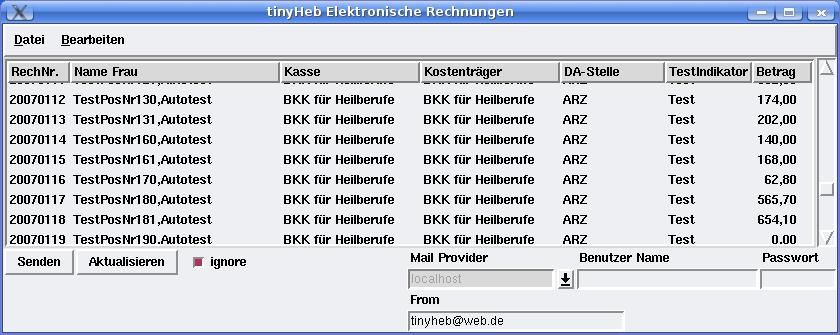
\includegraphics[width=80mm]{xauftrag}
\caption{Elektronische Rechnungen \label{kurz:xauftrag:fig}}
\end{figure}
Durch Anklicken einer Rechnungsnummer wird diese zum elektronischen Versand
ausgewählt. Über den Knopf \knopf{Senden} wird die Rechnung elektronisch
versand. Dabei wird die Rechnung sowohl an die entsprechende 
Datenannahmestelle geschickt, wie auch in Blindkopie an die Hebamme.
%
%
\section{Rechnungsbearbeitung}\label{kurz:rechnungsbearbeitung:kap}
Hat man eine oder mehrere Rechnungen erstellt, ist es notwendig, den
Zahlungseingang zu überwachen. Dazu dient die Maske 
\texttt{Rechnungsbearbeitung}. In diese Maske gelangt man aus dem
Hauptmenue über den Link \verb|versandte Rechnungen bearbeiten|.
Die Maske ist wie
auch die Maske Rechnungsgenerierung in zwei Teile gegliedert. Alle Rechnungen,
die bisher erstellt wurden, werden im oberen Teil der Maske angezeigt, dort
stehen zwei Knöpfe pro Rechnung zur Auswahl: 
% 
\begin{enumerate}[1.]
\item der Knopf \knopf{Bearbeiten}.
Über diesen Knopf werden die Daten der Rechnung
in den zweiten Teil der Maske übernommen. Dazu gehören insb. der Betrag
und der bisher gezahlte Betrag. Das Datum des
Rechnungseingangs und der gezahlte Betrag kann in den Feldern \feld{Zahldatum}
und \feld{Betrag gez.:} erfasst werden. Über den Knopf \knopf{Speichern}
werden die Daten gespeichert. Ist der bisher gezahlte Betrag und der aktuell
gezahlte Betrag kleiner als die ursprüngliche Rechnung, wird der Status auf
Teilzahlung gesetzt. Entspricht er der ursprünglichen Rechnung, bekommt diese
den Status erledigt.
\item der Knopf \knopf{Ansehen}.
Über diesen Knopf ist es möglich, sich
die original Rechnung anzusehen und bei Bedarf erneut zu drucken.
\end{enumerate}

Damit ist der komplette Zyklus einer Rechnung beschrieben. 
Details zur Erfassung von Stammdaten, Rechnungsposten, usw. 
finden sich in den nächsten Kapiteln.



%%% Local Variables: 
%%% mode: latex
%%% TeX-master: "anleitung"
%%% End: 
